\documentclass[conference]{IEEEtran}
\IEEEoverridecommandlockouts
\usepackage{cite}
\usepackage{amsmath,amssymb,amsfonts}
\usepackage{algorithmic}
\usepackage{graphicx}
\usepackage{textcomp}
\usepackage{xcolor}
\usepackage{hyperref}
\usepackage{booktabs}
\usepackage{enumitem}

\begin{document}

\title{Reading the Silicon: A Critical Visual Analysis of Hardware Fingerprints in Low-Light RAW Video}

\author{\IEEEauthorblockN{Keshav}
\IEEEauthorblockA{\textit{Netaji Subhas University of Technology} \\
New Delhi, India \\
keshav.ug25@nsut.ac.in}
}

\maketitle

\begin{abstract}
Digital image sensors operating under extreme low-light conditions produce imagery that is dominated not only by stochastic photon shot noise but also by a persistent, spatially structured layer of deterministic bias known as Fixed-Pattern Noise (FPN). This paper presents an empirical, graphical analysis of the stability, magnitude, and structural origins of FPN across 14 commercial smartphone camera modules, utilising the AIM 2025 Low-Light RAW Video dataset captured at approximately 1 lux. By extracting and systematically analysing FPN residual heatmaps, spatial Power Spectral Density (PSD) profiles, and hierarchical clustering dendrograms across five physically distinct scenes, the following principal findings are established. First, FPN constitutes an indelible, scene-independent topographical mask whose spatial structure is determined solely by the sensor hardware. Second, sharp harmonic spikes in row-wise PSD profiles implicate periodic column-parallel readout electronics as the dominant source of deterministic banding. Third, the RMS magnitude of FPN varies by a factor of approximately $22\times$ between modules housed within the same handset. Fourth, hierarchical clustering reveals that FPN structural similarity does not conform to brand-level grouping; cross-brand affinities instead suggest that the underlying sensor die and module type are more influential than manufacturer identity. These findings underscore the necessity of identifying and subtracting deterministic hardware signatures as a prerequisite to effective low-light image enhancement.
\end{abstract}

\begin{IEEEkeywords}
Fixed-Pattern Noise, Low-Light Video, RAW Sensor Data, Readout Architecture, Image Forensics
\end{IEEEkeywords}

\section{Introduction}

Extreme low-light videography places extraordinary demands on CMOS image sensors. At illumination levels approaching 1 lux, the incident photon flux is so severely attenuated that the genuine optical signal is frequently overwhelmed by noise contributions intrinsic to the sensor hardware \cite{el2005cmos, janesick2001scientific}. Among these, Fixed-Pattern Noise (FPN)---comprising spatially structured dark current non-uniformities and readout offset variations---constitutes a deterministic bias layer that persists identically across successive frames \cite{tian2001analysis, healey1994radiometric}. Unlike stochastic shot noise, which diminishes under temporal averaging, FPN remains as a rigid structural imprint of the silicon die and its associated readout circuitry.

\subsection{Limitations in the Existing Literature}

Despite extensive prior investigation, several important gaps persist in the current understanding of FPN behaviour under extreme low-light conditions:

\begin{enumerate}[label=(\roman*)]
    \item \textbf{Single-sensor forensic focus.} The seminal work of Lukas \textit{et al.} \cite{lukas2006digital} and subsequent large-scale studies \cite{goljan2009large, li2010source, fridrich2009digital} have convincingly demonstrated that Photo Response Non-Uniformity (PRNU) serves as a reliable camera fingerprint for forensic identification. However, these studies predominantly address the uniqueness of individual sensors rather than the \textit{structural relationships} between sensors from different manufacturers or module types.

    \item \textbf{Assumption of stochastic noise dominance.} Many state-of-the-art denoising pipelines---including learning-based approaches operating directly on RAW data \cite{chen2018learning, brooks2019unprocessing, wang2020practical}---implicitly treat sensor noise as predominantly stochastic. Physics-based noise models \cite{wei2020physics, foi2008practical, zhang2021rethinking} have begun to decompose noise into signal-dependent and signal-independent components, yet empirical characterisation of the deterministic FPN layer across diverse sensor populations remains limited.

    \item \textbf{Absence of cross-sensor comparative studies.} Existing FPN characterisation efforts \cite{konnik2014high, el2005cmos} typically examine individual sensors or sensor families in isolation. No prior study, to our knowledge, provides a systematic empirical comparison of FPN magnitude, spatial structure, and spectral characteristics across multiple camera modules from different manufacturers operating under identical controlled conditions.

    \item \textbf{Limited attention to intra-device variance.} Modern smartphones incorporate multiple camera modules (wide, ultrawide, telephoto, front-facing) within a single chassis. The extent to which FPN properties vary across co-located modules has not been systematically quantified, despite its direct relevance to multi-camera computational photography pipelines \cite{hasinoff2016burst}.
\end{enumerate}

\subsection{Contributions}

This work addresses the aforementioned limitations through a systematic, empirical investigation of FPN across 14 smartphone camera modules. The principal contributions are as follows:

\begin{enumerate}[label=(\arabic*)]
    \item A rigorous demonstration that FPN topographies are entirely scene-independent, persisting as identical spatial structures across five physically distinct scenes captured under controlled conditions.

    \item A quantitative characterisation of FPN magnitude across the full sensor fleet, revealing intra-device disparities of up to $22\times$ and establishing that noise severity is a property of the individual silicon die rather than the host device.

    \item A spectral analysis of FPN via row- and column-direction Power Spectral Density profiles, identifying sharp harmonic spikes that implicate periodic readout electronics as the primary source of deterministic banding artifacts.

    \item A hierarchical clustering analysis demonstrating that FPN structural similarity does not follow brand-level grouping, with cross-brand affinities suggesting shared upstream silicon components across manufacturers.
\end{enumerate}

\subsection{Paper Organisation}

The remainder of this paper is organised as follows. Section~II reviews related work on FPN characterisation, sensor forensics, and low-light denoising. Section~III describes the methodology employed to isolate deterministic hardware fingerprints from RAW sensor data. Section~IV presents the results and graphical analysis, encompassing FPN heatmaps, magnitude comparisons, temporal stability, spectral analysis, and cross-sensor clustering. Section~V discusses the implications, limitations, and directions for future work, and Section~VI concludes the paper.

\section{Related Work}

\subsection{Sensor Noise Characterisation}

Fixed-Pattern Noise arises from manufacturing variations in individual photodiodes and readout circuitry. Early characterisation by Healey and Kondepudy \cite{healey1994radiometric} established radiometric calibration procedures for CCD sensors, while El Gamal and Eltoukhy \cite{el2005cmos} provided a comprehensive treatment of noise sources in CMOS active pixel sensors. Tian \textit{et al.} \cite{tian2001analysis} analysed temporal noise contributions, distinguishing fixed offsets from frame-to-frame shot noise. The foundational physics of charge-coupled devices, including dark current generation mechanisms, are thoroughly documented by Janesick \cite{janesick2001scientific}. More recently, Konnik and Welsh \cite{konnik2014high} offered a unified tutorial on photosensor noise modelling spanning both CCD and CMOS architectures.

\subsection{Digital Forensics and Sensor Fingerprinting}

In digital forensics, Lukas \textit{et al.} \cite{lukas2006digital} demonstrated that PRNU---a multiplicative component of sensor noise---serves as a reliable camera fingerprint. Goljan \textit{et al.} \cite{goljan2009large} extended this to large-scale camera identification, and Li \cite{li2010source} proposed enhanced sensor pattern noise techniques for improved source camera identification. Fridrich \cite{fridrich2009digital} surveyed broader forensic applications, and Korus \cite{korus2017digital} provides a contemporary survey of image integrity verification techniques that build on these sensor-level signatures.

\subsection{Low-Light Denoising and Noise Modelling}

Physics-based noise models have gained prominence in the low-light regime. Foi \textit{et al.} \cite{foi2008practical} introduced a practical Poissonian-Gaussian framework for modelling noise in single-image RAW data. Wei \textit{et al.} \cite{wei2020physics} proposed a noise formation model specifically for extreme low-light RAW data, explicitly decomposing noise into signal-dependent shot noise and signal-independent fixed pattern components. Zhang \textit{et al.} \cite{zhang2021rethinking} re-examined noise synthesis strategies for RAW denoising pipelines, highlighting the importance of faithful noise characterisation.

On the algorithmic side, Chen \textit{et al.} \cite{chen2018learning} demonstrated end-to-end learning on RAW short-exposure imagery, while Hasinoff \textit{et al.} \cite{hasinoff2016burst} showed that burst averaging on mobile cameras suppresses temporal noise while preserving spatial detail. Abdelhamed \textit{et al.} \cite{abdelhamed2018high} contributed a high-quality benchmark dataset for smartphone camera denoising, and Brooks \textit{et al.} \cite{brooks2019unprocessing} proposed unprocessing natural images back to RAW for learned denoising. Fu \textit{et al.} \cite{fu2023low} addressed the specific challenge of low-light RAW video denoising with realistic motion, while Wang \textit{et al.} \cite{wang2020practical} demonstrated practical deep RAW denoising directly on mobile devices. Stripe-specific correction methods, such as the column drift compensation by Liu \textit{et al.} \cite{liu2014fixed} and the destriping framework by Bouali and Ladjal \cite{bouali2011detecting}, target the banding artifacts that are a primary manifestation of FPN.

Our work complements these approaches by providing an empirical, cross-sensor characterisation of FPN in a controlled multi-scene environment, focusing on the structural diversity and sensor-specificity of these patterns rather than proposing a correction algorithm.

\section{Methodology}

The objective of this study is to isolate and characterise the deterministic hardware fingerprints embedded in low-light RAW video. To achieve this, a strict analytical protocol was employed, operating exclusively on unprocessed sensor data without any Image Signal Processing (ISP), demosaicking, or machine learning enhancement. All analyses were conducted directly on native 10-bit and 12-bit RAW pixel values. The pipeline is summarised as follows.

\begin{enumerate}[label=\textbf{Step \arabic*:}, leftmargin=*, align=left]
    \item \textbf{Dataset and Frame Extraction.} The AIM 2025 Low-Light RAW Video Denoising Challenge dataset \cite{yakovenko2025aim} provides stop-motion RAW video captured at approximately 1 lux across 14 smartphone camera modules and five physically distinct scenes (coloured paper, hardware components, springs, toys, and yarn). All sequences were recorded on a motorised rail, ensuring perfect frame alignment and eliminating the need for software-based image registration.

    \item \textbf{Temporal Averaging.} For each sensor--scene pair, 10 contiguous noisy frames were temporally averaged at the individual pixel level using Welford's online algorithm \cite{konnik2014high}. This averaging suppresses stochastic shot noise by a factor of $\sqrt{10}$, progressively revealing the underlying deterministic bias.

    \item \textbf{Ground Truth Subtraction.} The resulting temporal mean still contains the actual optical scene content. To isolate the pure hardware contribution, the high-fidelity ground truth reference frame---a composite produced by the dataset authors from extended captures at the identical rail position---was subtracted from the temporal mean. The resulting residual matrix represents the deterministic offset injected by the sensor hardware.

    \item \textbf{Analytical Characterisation.} The extracted FPN residual maps were subjected to four complementary analyses: (a) spatial heatmap visualisation to assess scene independence, (b) RMS magnitude quantification across sensors, (c) Power Spectral Density computation in both row and column directions to identify periodic readout signatures, and (d) cross-sensor Pearson correlation and Ward-linkage hierarchical clustering to reveal structural affinities.
\end{enumerate}

All code and analysis scripts are publicly available.\footnote{\url{https://github.com/Keshav-poha/neural-archeology}}

\section{Results and Graphical Analysis}

This section presents the graphical outputs of the fingerprint extraction pipeline and analyses them systematically. Each subsection is organised around a specific analytical dimension, with figures presented alongside their interpretation.

\subsection{Scene Independence of FPN Topography}

Figure~\ref{fig:fpn_grid} presents bipolar heatmaps of the isolated FPN residuals for the 14 camera modules across all five scenes. Negative biases are mapped to blue and positive biases to red.

\begin{figure*}[t]
\centerline{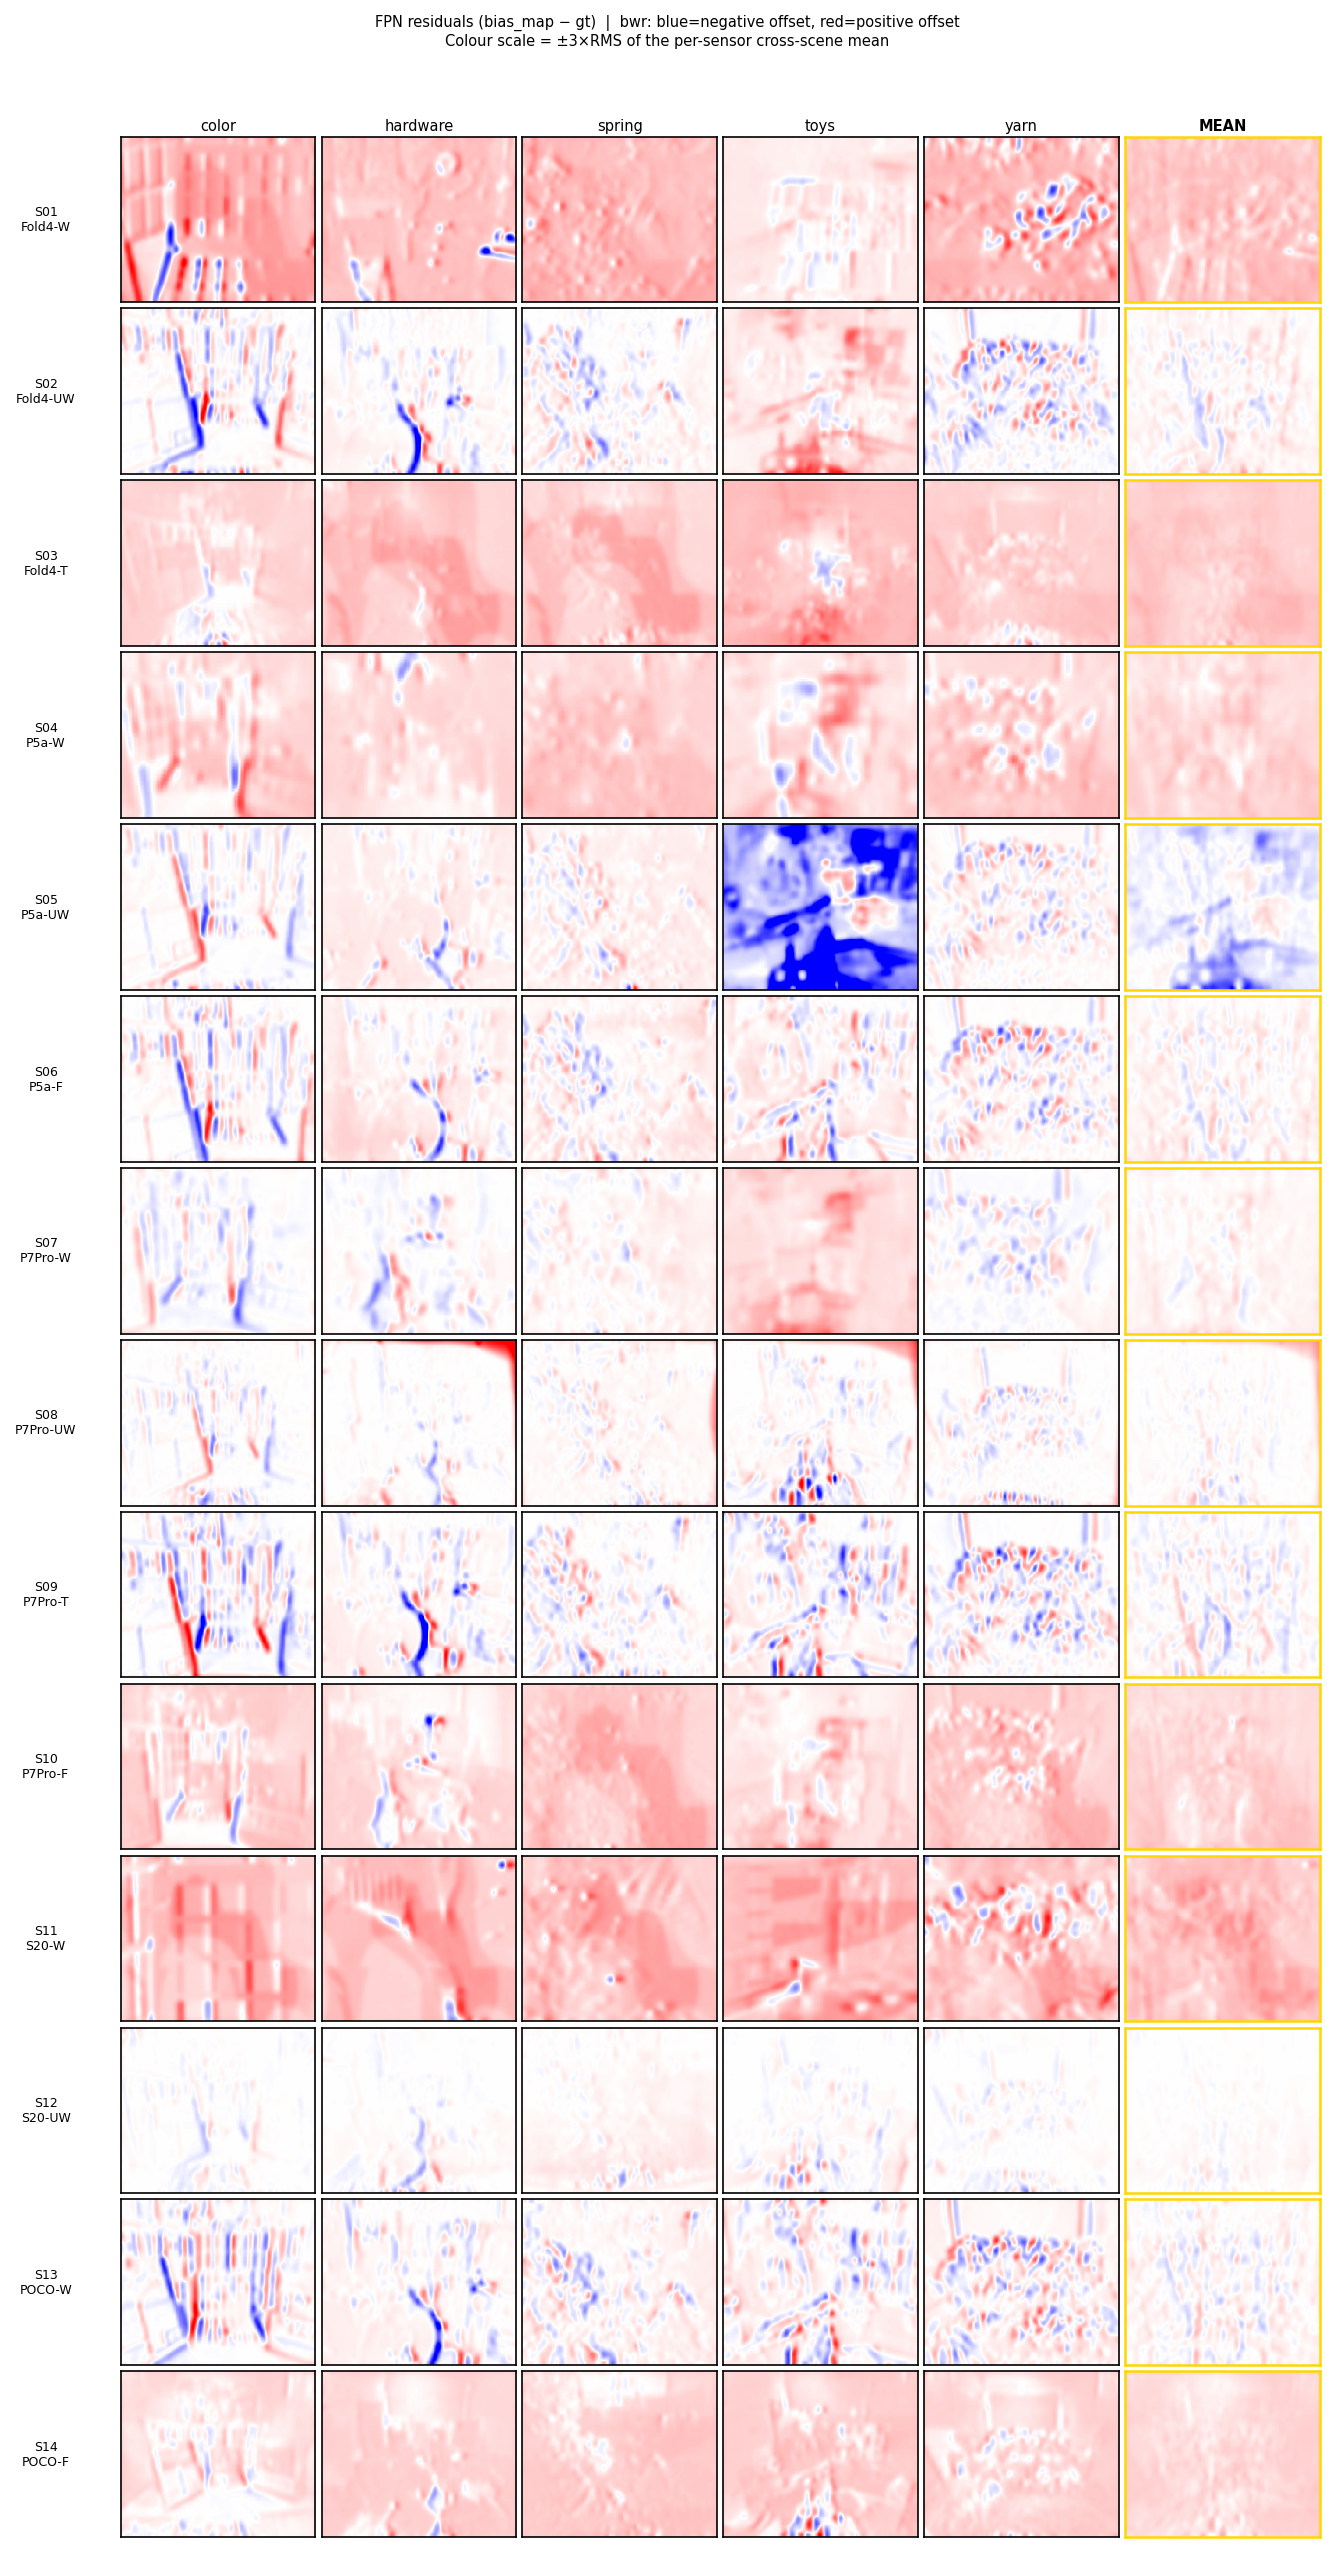
\includegraphics[width=\textwidth,height=0.85\textheight,keepaspectratio]{figures/fpn_overview.png}}
\caption{FPN residual heatmaps for the 14 camera modules across five scenes. Negative biases are mapped to blue, positive biases to red. The spatial structures---such as the deep negative pooling in the bottom-right quadrant of the Pixel 5a Ultrawide---remain rigidly locked at identical coordinates regardless of scene content.}
\label{fig:fpn_grid}
\end{figure*}

The FPN topography is demonstrably scene-independent. The Pixel 5a Ultrawide (Sensor~05) provides a particularly illustrative example: a pronounced region of negative bias localised in the bottom-right quadrant, paired with prominent vertical banding, persists identically whether the sensor is imaging coloured paper or an intricate collection of metal springs. This observation confirms that the extracted residuals represent intrinsic properties of the sensor's dark current distribution and readout offset structure \cite{el2005cmos, janesick2001scientific}, rather than optical artifacts. Because this deterministic map acts as a static overlay on every captured frame, it is amenable to calibration-based subtraction prior to any learning-based enhancement \cite{wei2020physics, brooks2019unprocessing}.

\subsection{FPN Magnitude Across the Sensor Fleet}

Figure~\ref{fig:fpn_mag} quantifies the mean RMS FPN magnitude per sensor, averaged across the five scenes. The complete per-sensor breakdown is provided in Table~\ref{tab:fpn_summary}.

\begin{figure}[t]
\centerline{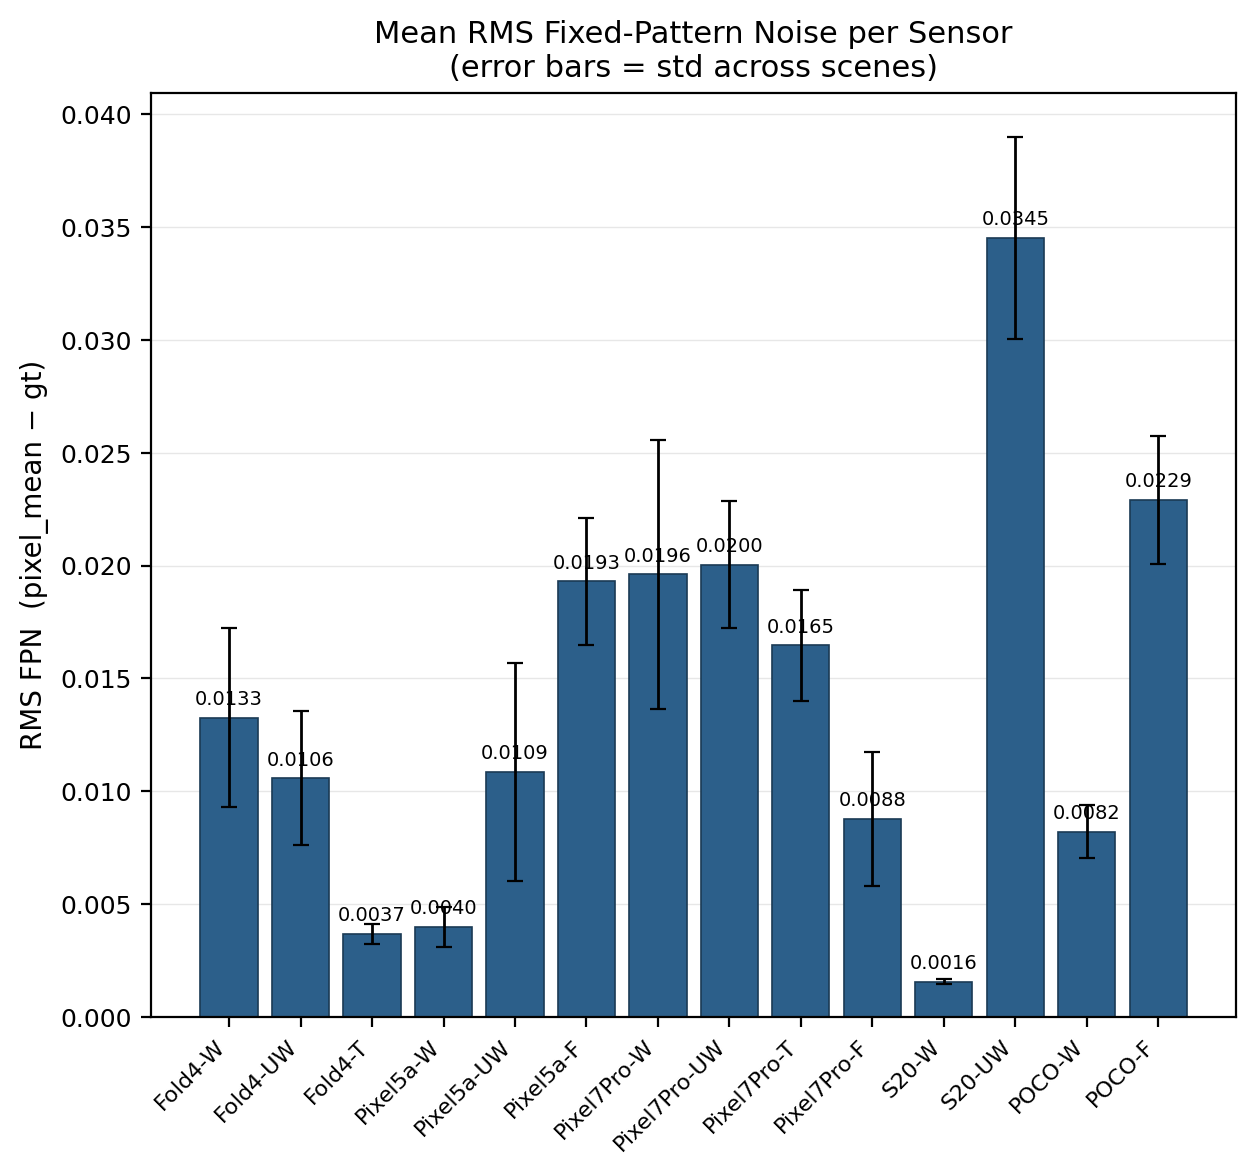
\includegraphics[width=\columnwidth]{figures/fpn_summary.png}}
\caption{Mean RMS Fixed-Pattern Noise per sensor (error bars indicate standard deviation across scenes). The S20 Ultrawide exhibits the highest FPN at approximately 0.035, while the S20 Wide registers near 0.002---a roughly $22\times$ disparity within the same handset.}
\label{fig:fpn_mag}
\end{figure}

\begin{table}[t]
\caption{Per-sensor FPN summary: mean RMS magnitude $\pm$ standard deviation across five scenes, sorted by descending magnitude.}
\label{tab:fpn_summary}
\centering
\small
\begin{tabular}{@{}llcc@{}}
\toprule
\textbf{\#} & \textbf{Module} & \textbf{RMS FPN} & \textbf{$\pm$ Std} \\
\midrule
12 & S20 UW        & 0.0345 & 0.0045 \\
14 & POCO Front    & 0.0229 & 0.0029 \\
 8 & P7Pro UW      & 0.0200 & 0.0028 \\
 7 & P7Pro W       & 0.0196 & 0.0060 \\
 6 & P5a Front     & 0.0193 & 0.0028 \\
 9 & P7Pro T       & 0.0165 & 0.0025 \\
 1 & Fold4 W       & 0.0133 & 0.0040 \\
 5 & P5a UW        & 0.0109 & 0.0048 \\
 2 & Fold4 UW      & 0.0106 & 0.0030 \\
10 & P7Pro Front   & 0.0088 & 0.0030 \\
13 & POCO W        & 0.0082 & 0.0012 \\
 4 & P5a W         & 0.0040 & 0.0009 \\
 3 & Fold4 T       & 0.0037 & 0.0005 \\
11 & S20 W         & 0.0016 & 0.0001 \\
\bottomrule
\end{tabular}
\end{table}

The S20 Ultrawide (S12) exhibits an RMS FPN of 0.0345, whereas the S20 Wide (S11)---a sensor housed within the same device---registers at just 0.0016. This approximately $22\times$ disparity within a single handset demonstrates conclusively that FPN severity is a property of the individual silicon die and its readout circuitry, not of the host device or its firmware. Other modules exhibiting elevated FPN include the POCO Front (0.0229) and the Pixel 7 Pro Ultrawide (0.0200), while the Fold4 Telephoto (0.0037) and S20 Wide (0.0016) remain comparatively pristine. These disparities have direct implications for multi-camera denoising pipelines \cite{wang2020practical}, where per-module calibration rather than per-device calibration is essential.

A further pattern emerges when FPN magnitudes are aggregated by module type. Across the sensor fleet, ultrawide modules exhibit a mean RMS FPN of 0.0190, approximately twice that of wide modules (0.0093). Front-facing modules average 0.0170, while telephoto modules average 0.0101. This disparity is physically plausible: ultrawide sensors typically employ larger dies with a greater number of column-parallel ADC channels \cite{el2005cmos}, amplifying the cumulative effect of per-column gain and offset variations on the overall FPN structure.

\subsection{Temporal Stability Under Varied Noise Regimes}

To evaluate whether the extracted fingerprints genuinely reflect intrinsic hardware properties, the mean pixel-wise temporal variance of the standard 10-frame noisy set was compared against a 20-frame extra-noisy validation set (Figure~\ref{fig:temp}).

\begin{figure}[t]
\centerline{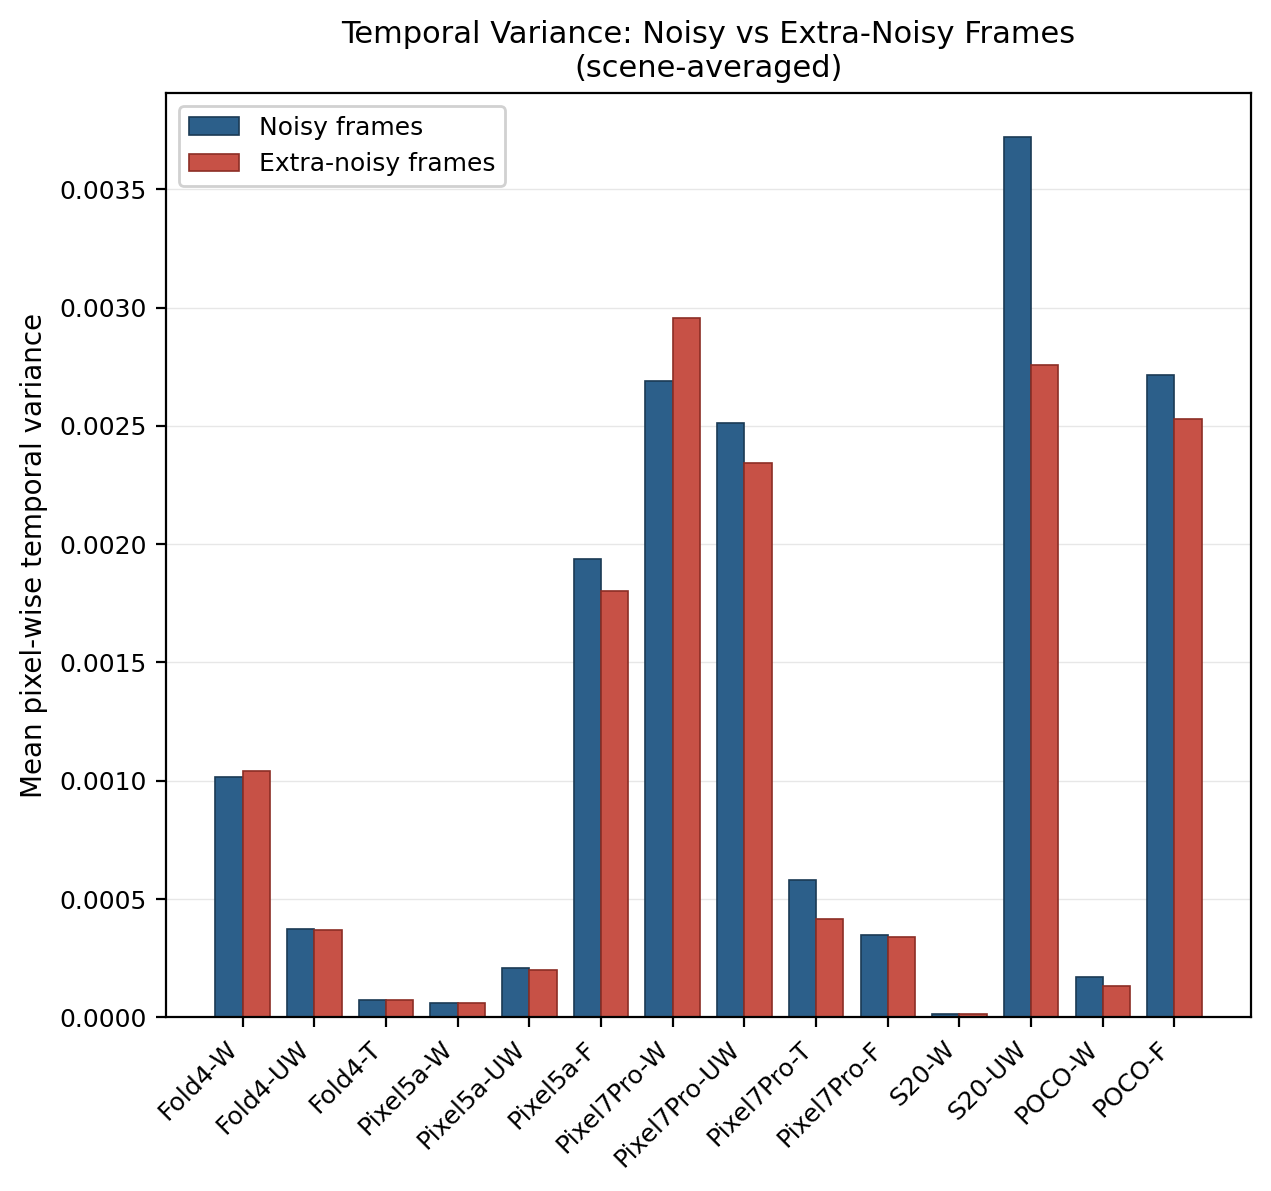
\includegraphics[width=\columnwidth]{figures/temporal_stability.png}}
\caption{Mean pixel-wise temporal variance: standard noisy frames (blue) versus extra-noisy frames (red) across the 14 sensors. The consistently higher variance in the standard set reflects the smaller averaging pool (10 vs.\ 20 frames).}
\label{fig:temp}
\end{figure}

As shown in Figure~\ref{fig:temp}, the blue bars (10-frame noisy set) are consistently taller than the red bars (20-frame extra-noisy set) for nearly every sensor. This result has a straightforward statistical explanation: the extra-noisy set averages over 20 frames, yielding variance estimates that benefit from a larger sample size and consequently converge more closely to the true expectation. The critical observation is that the \textit{relative ranking} of sensors is preserved across both conditions---modules exhibiting high variance under the standard set remain the highest under the extra-noisy set. This proportional stability confirms that the FPN derivation captures an intrinsic baseline property of the sensor hardware, invariant to the specific noise realisation.

\subsection{Spectral Analysis of Readout Architecture}

To elucidate the directional structure of the deterministic artifacts, Power Spectral Density (PSD) profiles were computed along the horizontal (row) and vertical (column) axes of the FPN residual matrices (Figures~\ref{fig:psd} and~\ref{fig:col_psd}).

\begin{figure}[t]
\centerline{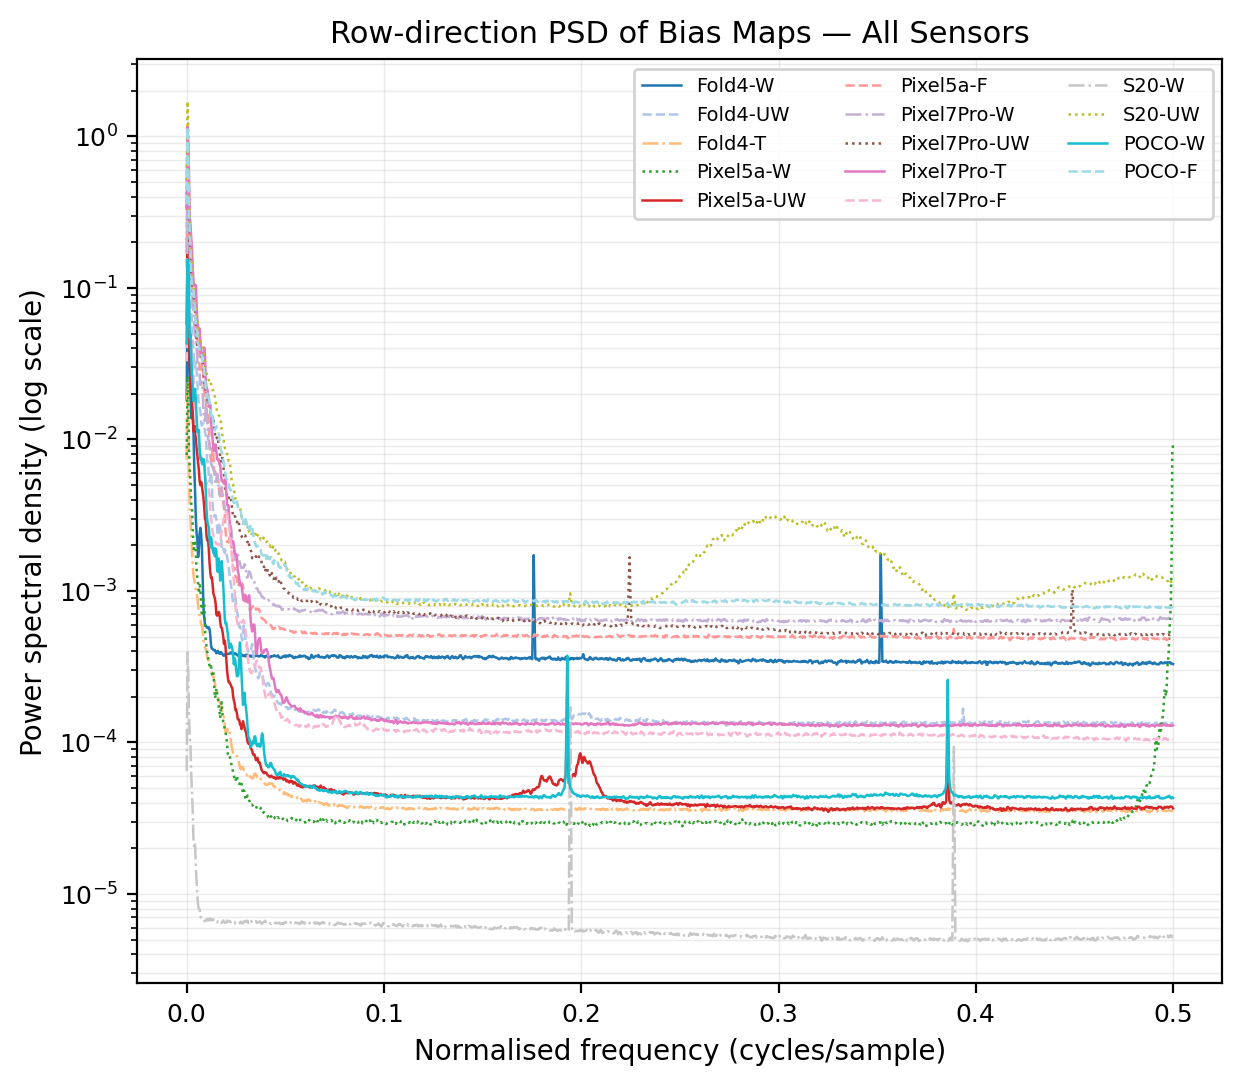
\includegraphics[width=\columnwidth]{figures/row_psd.png}}
\caption{Row-direction Power Spectral Density (PSD) of the FPN residuals. Sharp harmonic spikes are visible at discrete normalised frequencies, particularly from the S20 Wide, Fold4 Wide, and POCO Wide modules.}
\label{fig:psd}
\end{figure}

In a purely random noise field, the spatial frequency spectrum would present as a smooth, featureless curve. Instead, the row-wise PSDs reveal sharp harmonic spikes at distinct normalised frequencies. The S20 Wide exhibits the most prominent spikes at approximately 0.2 and 0.4 cycles/sample, while the Fold4 Wide shows a clear peak near 0.19 cycles/sample. The Pixel 5a Wide dominates the low-frequency region with a PSD magnitude roughly an order of magnitude above most other sensors, indicating large-scale spatial non-uniformity rather than fine-grained periodic banding. These resonant peaks correspond to perfectly periodic stripes embedded in the sensor output, consistent with systematic variations in column-parallel ADC behaviour and shared readout amplifiers \cite{el2005cmos, liu2014fixed}.

\begin{figure}[t]
\centerline{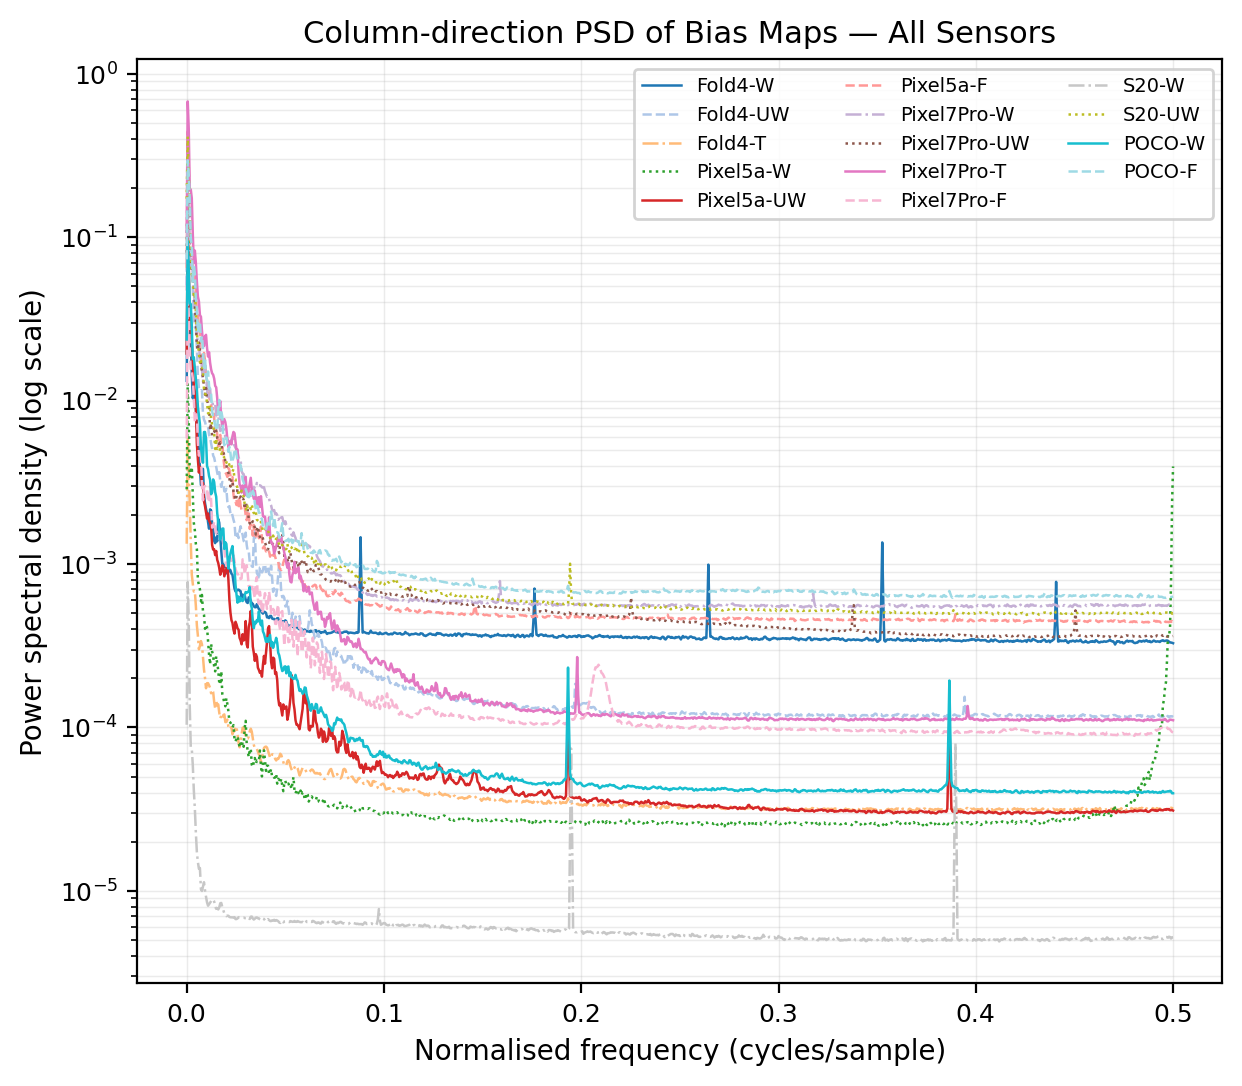
\includegraphics[width=\columnwidth]{figures/col_psd.png}}
\caption{Column-direction PSD of the FPN residuals. While generally exhibiting a flatter profile than the row direction, several sensors display localised spikes, indicating that readout artifacts are not exclusively row-aligned.}
\label{fig:col_psd}
\end{figure}

The column-direction PSD (Figure~\ref{fig:col_psd}) reveals that while the row direction hosts the most prominent harmonic structure, the column direction is not entirely featureless: the Fold4 Wide exhibits a spike near 0.08 cycles/sample, and the Pixel 5a Wide rises sharply at the Nyquist boundary. This indicates that banding is primarily row-aligned---consistent with row-sequential readout and shared column amplifiers---but a secondary column-wise component exists in certain sensor architectures.

\subsection{Cross-Sensor Structural Affinities}

To investigate manufacturing-level relationships among the 14 modules, a cross-sensor Pearson correlation matrix was computed from scene-averaged FPN maps (Figure~\ref{fig:similarity}), and Ward-linkage hierarchical clustering was applied to the corresponding Euclidean distance matrix (Figure~\ref{fig:dendrogram}).

\begin{figure}[t]
\centerline{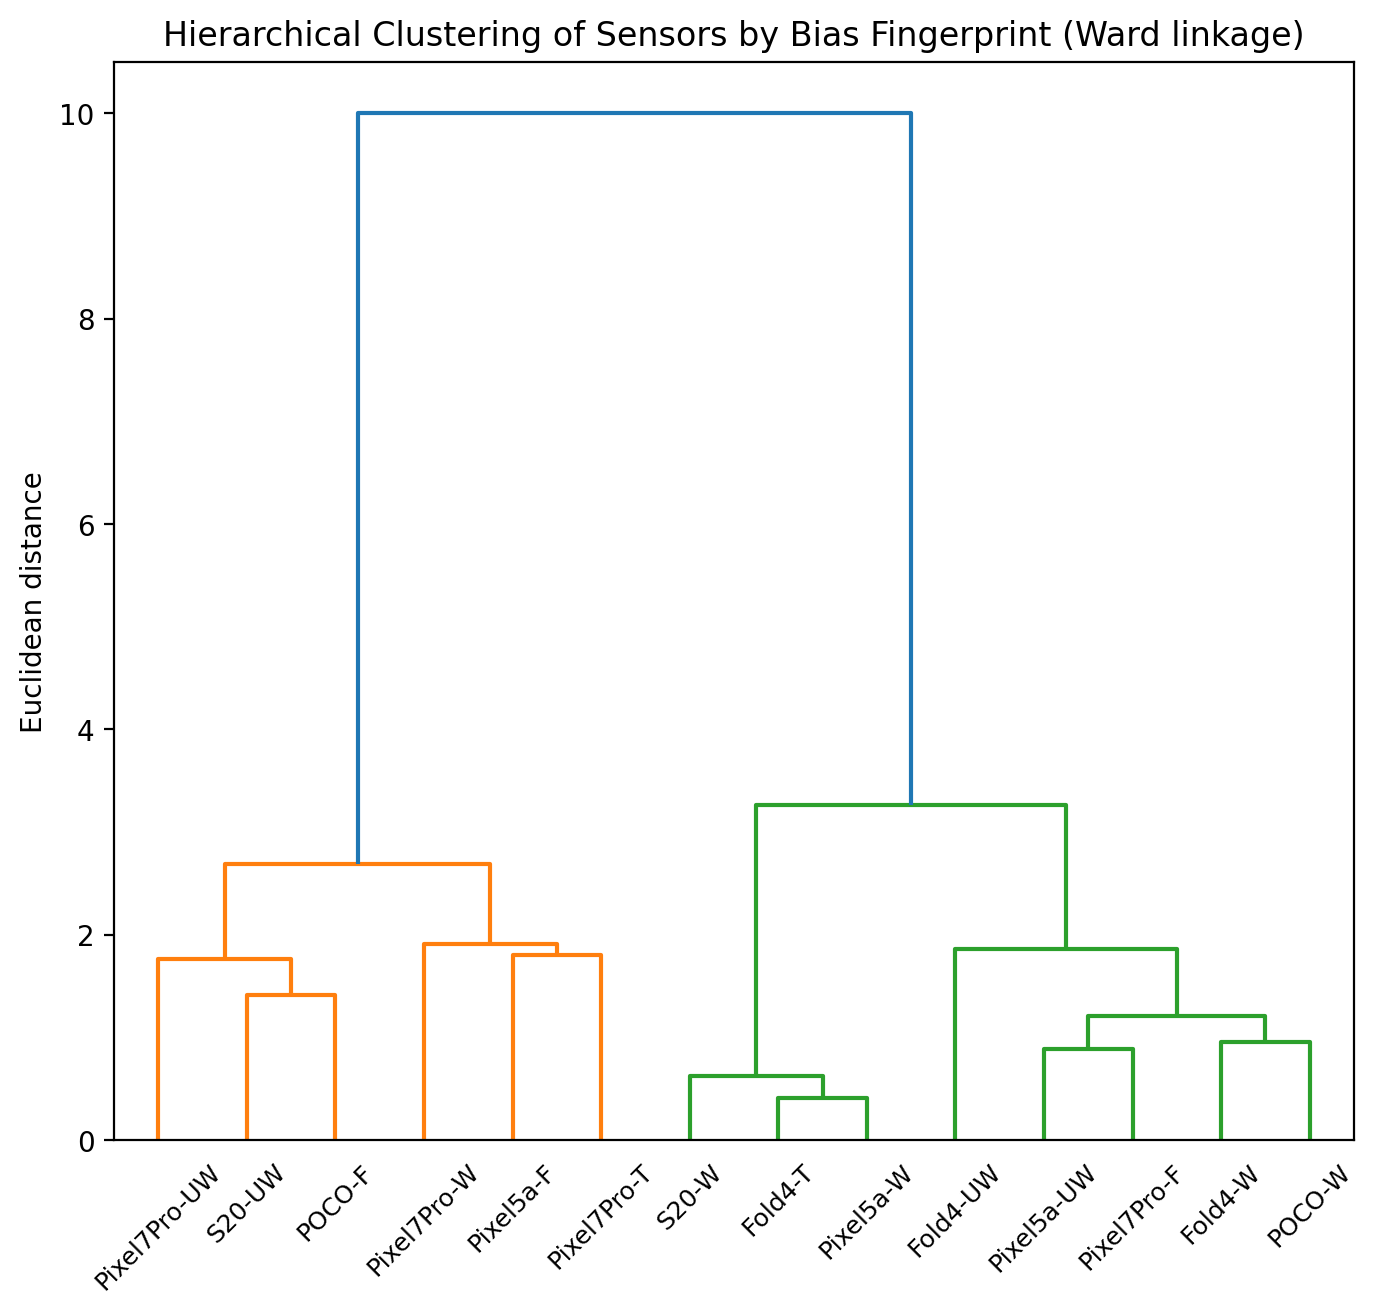
\includegraphics[width=\columnwidth]{figures/sensor_dendrogram.png}}
\caption{Dendrogram clustering the 14 modules by FPN structural similarity (Ward linkage). The dendrogram splits into two macro-branches (orange, green) at a Euclidean distance of approximately 10, each containing a heterogeneous mixture of brands and module types.}
\label{fig:dendrogram}
\end{figure}

The dendrogram (Figure~\ref{fig:dendrogram}) reveals a far more nuanced structure than simple brand-level grouping would suggest. The tree splits into two macro-branches at a Euclidean distance of approximately 10. The left branch groups the Pixel 7 Pro Ultrawide with the S20 Ultrawide and the POCO Front---three modules from three distinct manufacturers. The right branch is equally heterogeneous, pairing the S20 Wide with the Fold4 Telephoto at a strikingly low linkage distance ($\sim$0.4) and grouping Pixel 5a modules alongside the Fold4 Ultrawide, Pixel 7 Pro Front, Fold4 Wide, and POCO Wide.

\begin{figure}[t]
\centerline{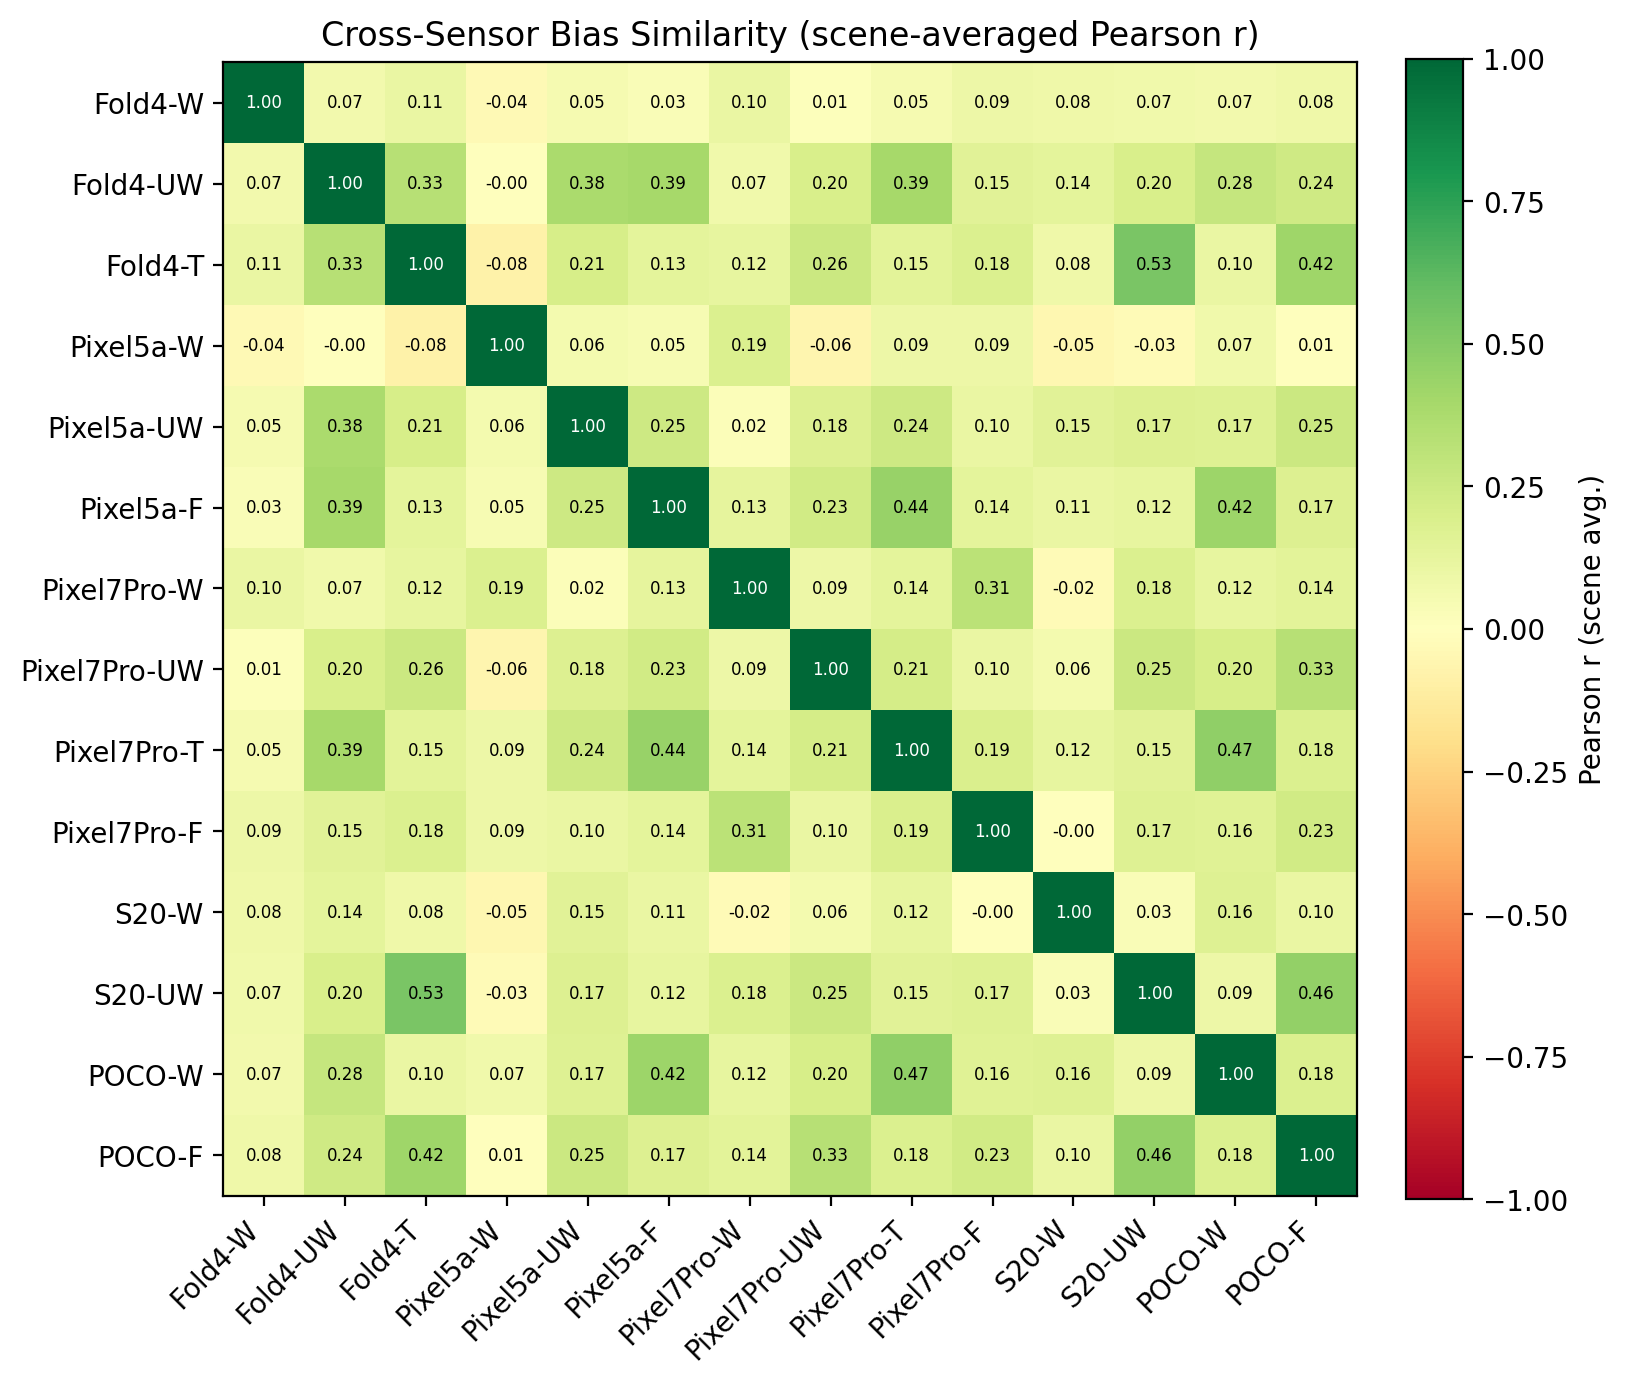
\includegraphics[width=\columnwidth]{figures/sensor_similarity.png}}
\caption{Cross-sensor Pearson similarity matrix (scene-averaged). The highest off-diagonal correlation ($r = 0.53$) occurs between the Fold4 Telephoto and S20 Ultrawide, two modules from different Samsung handsets released years apart.}
\label{fig:similarity}
\end{figure}

Two principal patterns emerge from this analysis. First, while several Pixel modules cluster in proximity, the Pixel family is distributed across \textit{both} macro-branches, indicating that module type (wide, ultrawide, telephoto, front-facing) and the underlying sensor die exert greater influence on FPN structure than brand identity alone. Second, strong cross-brand pairings appear consistently: the S20 Wide and Fold4 Telephoto merge at very low linkage distance, and the Pixel 7 Pro Ultrawide clusters with the S20 Ultrawide.

The similarity matrix (Figure~\ref{fig:similarity}) provides complementary quantitative evidence. The highest off-diagonal Pearson correlation ($r = 0.53$) is between the Fold4 Telephoto (S03) and S20 Ultrawide (S12)---two modules from entirely different Samsung devices released years apart. Other elevated correlations include POCO Wide vs.\ Pixel 7 Pro Telephoto ($r = 0.47$) and Pixel 5a Front vs.\ Pixel 7 Pro Telephoto ($r = 0.44$). Both the dendrogram (Ward linkage on Euclidean distance) and the similarity matrix (Pearson correlation) consistently demonstrate cross-brand structural affinities, which is compatible with the hypothesis that certain modules share upstream silicon from a common supplier---though the present data alone cannot confirm this causal mechanism.

\subsection{Summary of Findings}

The analyses presented above yield five principal empirical findings:

\begin{enumerate}[label=(\arabic*)]
    \item \textbf{Scene independence:} FPN topographies are unambiguously scene-independent; identical spatial structures persist across five physically distinct scenes (Figure~\ref{fig:fpn_grid}).

    \item \textbf{Intra-device magnitude disparity:} FPN severity varies by more than $20\times$ within a single handset (Table~\ref{tab:fpn_summary}), demonstrating that noise characteristics are properties of the individual sensor die, not the host device.

    \item \textbf{Module-type dependence:} When grouped by optical role, ultrawide modules exhibit approximately twice the mean RMS FPN of wide modules (0.0190 vs.\ 0.0093), consistent with the larger die area and greater number of column-parallel readout channels in ultrawide sensors.

    \item \textbf{Readout-driven periodicity:} Sharp harmonic spikes in row-wise PSD profiles consistently implicate periodic readout circuitry as the primary driver of deterministic banding (Figures~\ref{fig:psd} and~\ref{fig:col_psd}).

    \item \textbf{Cross-brand structural affinities:} Hierarchical clustering and cross-sensor correlation reveal unexpected structural similarities across manufacturers and device generations, suggesting shared upstream silicon components (Figures~\ref{fig:dendrogram} and~\ref{fig:similarity}).
\end{enumerate}

\section{Discussion and Limitations}

The findings of this study carry direct implications for low-light computational photography pipelines \cite{chen2018learning, hasinoff2016burst, fu2023low}. Because FPN is deterministic and scene-independent, it is amenable to calibration-based subtraction as a pre-processing step, isolating the stochastic noise component for downstream algorithms. The substantial intra-device FPN disparities further imply that per-module calibration is essential; device-level correction would be insufficient for multi-camera systems. The observation that ultrawide modules consistently exhibit approximately twice the FPN of their wide counterparts suggests that module-type-aware calibration strategies may be warranted, with ultrawide sensors requiring more aggressive correction. The cross-brand structural affinities uncovered by the clustering analysis suggest that module-level rather than brand-level noise models may be more appropriate for generalised denoising frameworks \cite{zhang2021rethinking, abdelhamed2018high}.

Several limitations must be acknowledged. This study examines only 14 sensor modules from 5 smartphones, all operating at a single illumination level ($\sim$1 lux). Whether these fingerprints exhibit identical behaviour at higher illumination levels, different frame rates, or varying ambient temperatures remains unverified. Additionally, the sensor numbering used throughout this work is \textit{inferred} from the column order of the challenge paper's performance table; the dataset does not publish an official numeric-to-model mapping. The 10-frame temporal average, while substantially suppressing shot noise, does not eliminate it entirely; residual stochastic contamination may slightly inflate the measured FPN magnitudes. Finally, while the cross-brand clustering results are suggestive of shared upstream silicon suppliers, confirming this hypothesis would require access to detailed sensor specifications that are not publicly available.

\section{Conclusion}

Fixed-Pattern Noise in extreme low-light RAW video is not a random nuisance---it is a spatially structured, highly sensor-specific architectural signature that persists rigidly across varying scene content. The empirical evidence presented in this study demonstrates that these hardware fingerprints maintain proportional stability under different noise regimes and reveal unexpected structural affinities across manufacturers through hierarchical clustering.

For computational photography, the implication is clear: any denoising pipeline operating on 1-lux RAW video should first identify and subtract this deterministic hardware bias before attempting to recover the genuine optical signal. Whether scene-independent correction functions can be derived entirely without ISP operations---and whether such corrections generalise across illumination levels and sensor temperatures---remains an important direction for future investigation.

\section*{Acknowledgment}

The author wishes to acknowledge the structural foundation provided by the AIM 2025 extreme low-light dataset challenge. We also express our sincere gratitude to Dr. Ankush Jain, Assistant Professor in the Department of Computer Science and Engineering at Netaji Subhas University of Technology (NSUT), for his insightful review and valuable suggestions which significantly improved the quality of this work.

\bibliographystyle{IEEEtran}
\bibliography{references}

\end{document}
